\section{Hidden Markov Chain (HMC)}
\label{sec:datasets-hmc}

The HMC dataset is a synthetic sequence-labeling task on a
linear-chain graph. It plays a supporting role in this thesis: it
is the testbed on which the LP-relaxed M\textsuperscript{3}N
training loss can be compared against exact structured-hinge
training, since on chains exact loss-augmented inference is
available via Viterbi (Section~\ref{subsec:viterbi}). Sequences
have length $T = 30$ over $K = 10$ states; full generation
parameters are given in Section~\ref{subsec:hmc-generation}.

\subsection{Generation procedure}
\label{subsec:hmc-generation}

The data generator produces sequences of length $T$ over a label
set of size $K$. The hidden state $y_t \in \{0, \ldots, K-1\}$
follows a $K$-state Markov chain with a uniform initial
distribution and a self-transition kernel
\begin{equation}
    \mathbb{P}(y_t = y_{t-1}) = p_{\mathrm{self}},
    \qquad
    \mathbb{P}(y_t = j \mid y_{t-1} = i,\ j \neq i)
    = \frac{1 - p_{\mathrm{self}}}{K - 1}.
    \label{eq:hmc-transition}
\end{equation}
The observation $x_t \in \{0, \ldots, K-1\}$ is a noisy emission
of $y_t$ governed by
\begin{equation}
    \mathbb{P}(x_t = y_t) = p_{\mathrm{emit}},
    \qquad
    \mathbb{P}(x_t = j \mid y_t = i,\ j \neq i)
    = \frac{1 - p_{\mathrm{emit}}}{K - 1}.
    \label{eq:hmc-emission}
\end{equation}
Both the transition and the emission kernels are doubly
stochastic: every off-diagonal probability mass is split equally
across the $K - 1$ alternative classes. The default
configuration is $T = 30$, $K = 10$,
$p_{\mathrm{self}} = 0.7$, $p_{\mathrm{emit}} = 0.7$.

The library function
\texttt{generate\_hmc\_sequences(N, T, K, p\_self, p\_emit, seed)}
produces $N$ sequences and returns two arrays:
\texttt{obs\_indices} of shape $[N, T]$ and \texttt{labels} of
shape $[N, T]$.

\subsection{Symbolic and visual variants}
\label{subsec:hmc-variants}

All sequences in the benchmark share the same fixed length
$T = 30$, so the tensor shapes below are uniform across the
dataset.

\paragraph{Symbolic.}
Per-step one-hot encoding of the observation index: each
$x_t$ becomes a $K$-dimensional vector with a $1$ at index $x_t$.
The input tensor has shape $\mathbb{R}^{T \times K}$ and the
output is $y \in \{0, \ldots, K-1\}^{T}$.

\paragraph{Visual.}
Each $x_t$ is replaced by a randomly sampled MNIST image of the
digit $x_t$, drawn from the per-split image pool
(Section~\ref{subsec:hmc-splits}). The input tensor has shape
$\mathbb{R}^{T \times 1 \times 28 \times 28}$.

Figure~\ref{fig:hmc-symbolic-example} renders one symbolic
training sequence as a two-row strip: $x_t$ on top, $y_t$
underneath, with cells where the emission noise has corrupted the
observation ($x_t \neq y_t$) shaded in red. The visual analogue
is shown in Figure~\ref{fig:hmc-visual-example}, with MNIST
images on top and a red border on the cells where emission noise
was applied.

\begin{figure}[htbp]
\centering
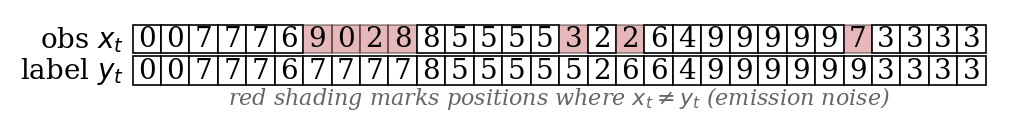
\includegraphics[width=\textwidth]{figures/data/hmc_symbolic_example}
\caption[Symbolic HMC example]{One symbolic HMC training
sequence; red shading marks emission noise ($x_t \neq y_t$).}
\label{fig:hmc-symbolic-example}
\end{figure}

\begin{figure}[htbp]
\centering
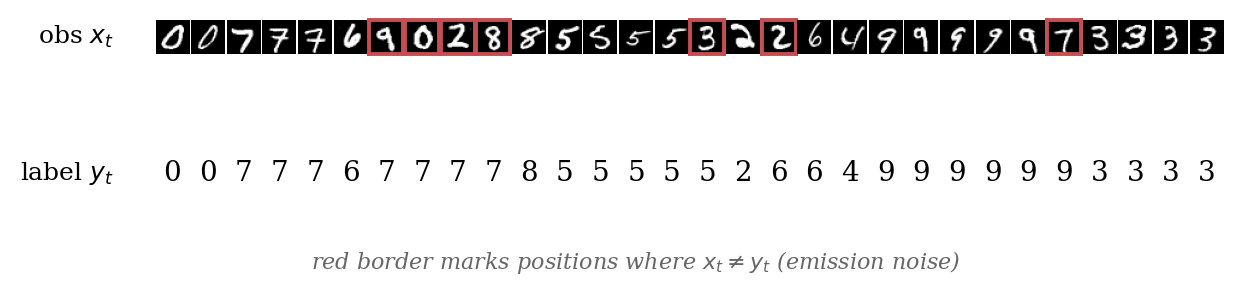
\includegraphics[width=\textwidth]{figures/data/hmc_visual_example}
\caption[Visual HMC example]{Visual rendering of a training
sequence; red borders mark cells where emission noise was applied.}
\label{fig:hmc-visual-example}
\end{figure}

\subsection{Splits and reproducibility}
\label{subsec:hmc-splits}

A total of $50{,}000$ sequences are generated with the seed
\texttt{hmc\_seed = 42} and split into $30{,}000$ training,
$10{,}000$ validation, and $10{,}000$ test sequences.

The visual variant uses the same disjoint-MNIST-pool scheme as
Sudoku: train and val draw from disjoint partitions of the MNIST
training set ($75\% / 25\%$ split per digit class), and test
draws from the MNIST test set. The image-index assignment uses
\texttt{mnist\_seed = 123} with offsets $+0$, $+1$, $+2$ for
train, val, and test. All seeds are stored in
\texttt{config.json}.

\subsection{Statistics and role}
\label{subsec:hmc-stats}

\paragraph{Empirical kernel parameters.}
On the training split, the empirical self-transition rate is
$\hat p_{\mathrm{self}} = 0.7000$ and the empirical correct-emission
rate is $\hat p_{\mathrm{emit}} = 0.7008$, both within sampling
noise of the configured $0.7$.

\paragraph{Marginal state distribution.}
The marginal state distribution is approximately uniform with
$\hat{\mathbb{P}}(y_t = i) \approx 1/K = 0.1$ for every $i$, as
expected from the doubly stochastic transition kernel and uniform
initial state.

\paragraph{Transition structure.}
Figure~\ref{fig:hmc-transition} shows the empirical transition
matrix: a diagonal-heavy structure with
$\hat{\mathbb{P}}(y_{t+1} = i \mid y_t = i) \approx p_{\mathrm{self}}$
on the diagonal and $\approx (1 - p_{\mathrm{self}}) / (K - 1)$
off-diagonal, matching the construction in
Eq.~\eqref{eq:hmc-transition}.

\begin{figure}[htbp]
\centering
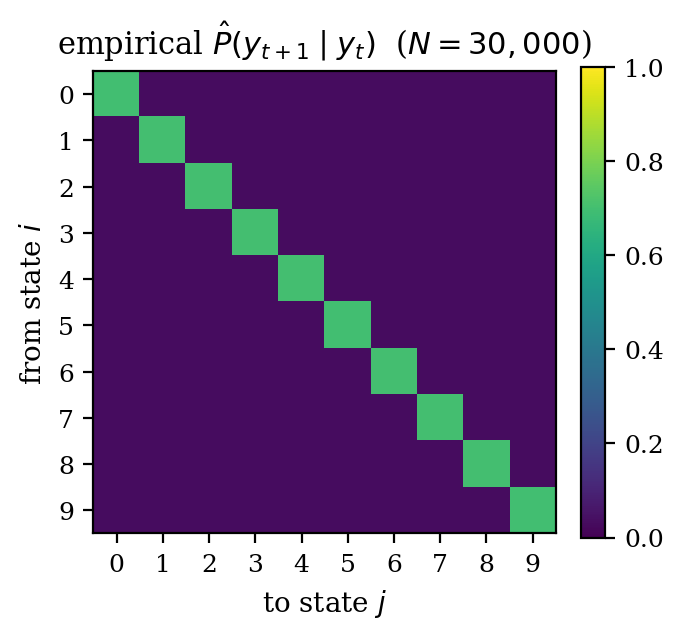
\includegraphics[width=0.55\textwidth]{figures/data/hmc_transition}
\caption[HMC transition matrix]{Empirical transition matrix on the
HMC training split.}
\label{fig:hmc-transition}
\end{figure}

\paragraph{MNIST-pool reuse.}
The MNIST-pool reuse pattern for HMC is shown in
Figure~\ref{fig:hmc-mnist-pool-usage}; the analysis is analogous
to the Sudoku case (Figure~\ref{fig:sudoku-mnist-pool-usage}).

\begin{figure}[htbp]
\centering
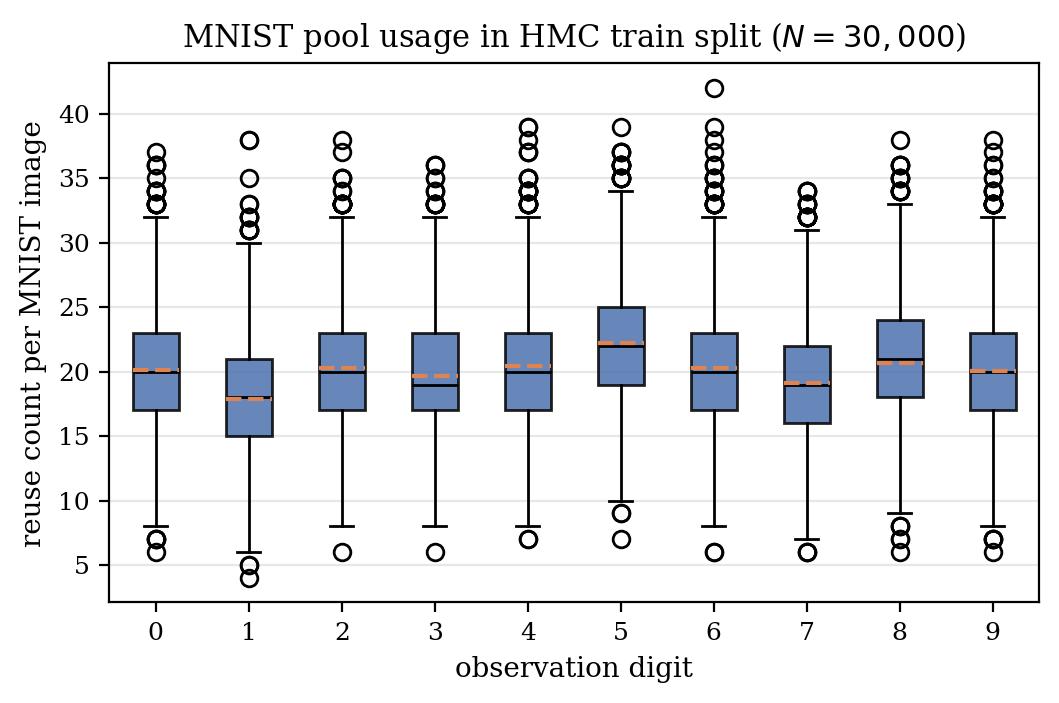
\includegraphics[width=0.85\textwidth]{figures/data/hmc_mnist_pool_usage}
\caption[HMC MNIST pool usage]{Per-state reuse counts of
training-split MNIST images, HMC visual variant.}
\label{fig:hmc-mnist-pool-usage}
\end{figure}

\paragraph{Role.}
Because the LP relaxation is exact on trees
(Section~\ref{subsec:lp-relaxation}), on a chain the LP-relaxed
M\textsuperscript{3}N learning loss must coincide with the exact
structured-hinge training of Section~\ref{subsec:structured-hinge}.
Chapter~\ref{chap:experiments} reports this comparison and uses
agreement on HMC as a correctness anchor for the LP-M3N
implementation.
